\documentclass{scrartcl}
\usepackage{graphicx}
\usepackage{amsmath}
\usepackage{listings}
\usepackage{mathtools}
\usepackage{physics}
\usepackage{siunitx}
\usepackage{tikz}
\usepackage{mathtools}
\usepackage{rotating}
\usepackage{hyperref}
\usepackage{fancyhdr}
\usepackage{float}

\pagestyle{fancy}
\fancyhf{}
\rhead{Jamie Grieser}
\lhead{Simulation Methods}
\rfoot{Page \thepage}

\definecolor{mygreen}{rgb}{0,0.6,0}
\definecolor{mygray}{rgb}{0.5,0.5,0.5}
\definecolor{mymauve}{rgb}{0.58,0,0.82}

\lstset{ 
	backgroundcolor=\color{white},   % choose the background color; you must add \usepackage{color} or \usepackage{xcolor}; should come as last argument
	basicstyle=\footnotesize,        % the size of the fonts that are used for the code
	breakatwhitespace=false,         % sets if automatic breaks should only happen at whitespace
	breaklines=true,                 % sets automatic line breaking
	captionpos=b,                    % sets the caption-position to bottom
	commentstyle=\color{mygreen},    % comment style
	deletekeywords={...},            % if you want to delete keywords from the given language
	escapeinside={\%*}{*)},          % if you want to add LaTeX within your code
	extendedchars=true,              % lets you use non-ASCII characters; for 8-bits encodings only, does not work with UTF-8
	frame=single,	                   % adds a frame around the code
	keepspaces=false,                 % keeps spaces in text, useful for keeping indentation of code (possibly needs columns=flexible)
	keywordstyle=\color{blue},       % keyword style
	language=Octave,                 % the language of the code
	morekeywords={*,...},            % if you want to add more keywords to the set
	numbers=left,                    % where to put the line-numbers; possible values are (none, left, right)
	numbersep=5pt,                   % how far the line-numbers are from the code
	numberstyle=\tiny\color{mygray}, % the style that is used for the line-numbers
	rulecolor=\color{black},         % if not set, the frame-color may be changed on line-breaks within not-black text (e.g. comments (green here))
	%showspaces=false,                % show spaces everywhere adding particular underscores; it overrides 'showstringspaces'
	showstringspaces=false,          % underline spaces within strings only
	showtabs=false,                  % show tabs within strings adding particular underscores
	stepnumber=2,                    % the step between two line-numbers. If it's 1, each line will be numbered
	stringstyle=\color{mymauve},     % string literal style
	tabsize=2,	                   % sets default tabsize to 2 spaces
	%title=\lstname                   % show the filename of files included with \lstinputlisting; also try caption instead of title
}

\begin{document}

\section*{Problem Sheet 8}
\subsection*{Exercise 1.1}
We begin the discussion of the exercise with the functions for the symmetric and upwind numerical differential operators. The field with initial and boundary conditions is initialized using the following function:
\begin{lstlisting}[title=Function to initialize boundary and initial conditions on the field.,  language=Python, frame=single]
# Function to create a vector that contains the discrete values of the field
def create_field(dimension, left_boundary, right_boundary, length):
	u = np.zeros((dimension + 2, 1))
	for i in range(1, dimension + 1):
		dist = i * dx - length / 2
		if dist < 0:
		u[i] = 1
	u[0] = left_boundary
	u[dimension + 1] = right_boundary
	return u, dimension
\end{lstlisting}
The implementation of the algorithms for the symmetric and upwind operators is shown below:
\begin{lstlisting}[title=Symmetric numerical derivative code.,  language=Python, frame=single]
def symmetric_scheme(left_boundary, right_boundary):
	u, dim = create_field(100, left_boundary, right_boundary, L)
	v = velocity(shape='constant', dimension=dim)
	for i in range(0, timesteps):
		for j in range(1, dim):
			u[j] = u[j] - v[j] * (u[j+1] - u[j-1])/(2*dx) * dt
	return u
\end{lstlisting}
\begin{lstlisting}[title=Upwind numerical derivative code.,  language=Python, frame=single]
def upwind_scheme(left_boundary, right_boundary):
	u, dim = create_field(100, left_boundary, right_boundary, L)
	v = velocity(shape='constant', dimension=dim)
	for i in range(0, timesteps):
		for j in range(1, dim):
			u[j] = u[j] - v[j] * (u[j] - u[j - 1]) / dx * dt
	return u
\end{lstlisting}
In figure \ref{fig:symmetricandupwind}, we can see the plots of this functions. One immediately sees the oscillation of the numerical instability for the symmetric schemes.
Figure \ref{fig:upwindunstable} displays the unstable upwind algorithm which was computed using the following function:
\begin{lstlisting}[title=Upwind numerical derivative code with shifted indices. This will lead to numerical instabilities.,  language=Python, frame=single]
# Implementing the upwind scheme with the index shift
def upwind_scheme_reversed(left_boundary, right_boundary):
	u, dim = create_field(100, left_boundary, right_boundary, L)
	v = velocity(shape='constant', dimension=dim)
	for i in range(0, timesteps):
		for j in range(2, dim):
			u[j] = u[j] - v[j] * (u[j + 1] - u[j]) / dx * dt
	return u
\end{lstlisting}
\begin{figure}[H]
	\centering
	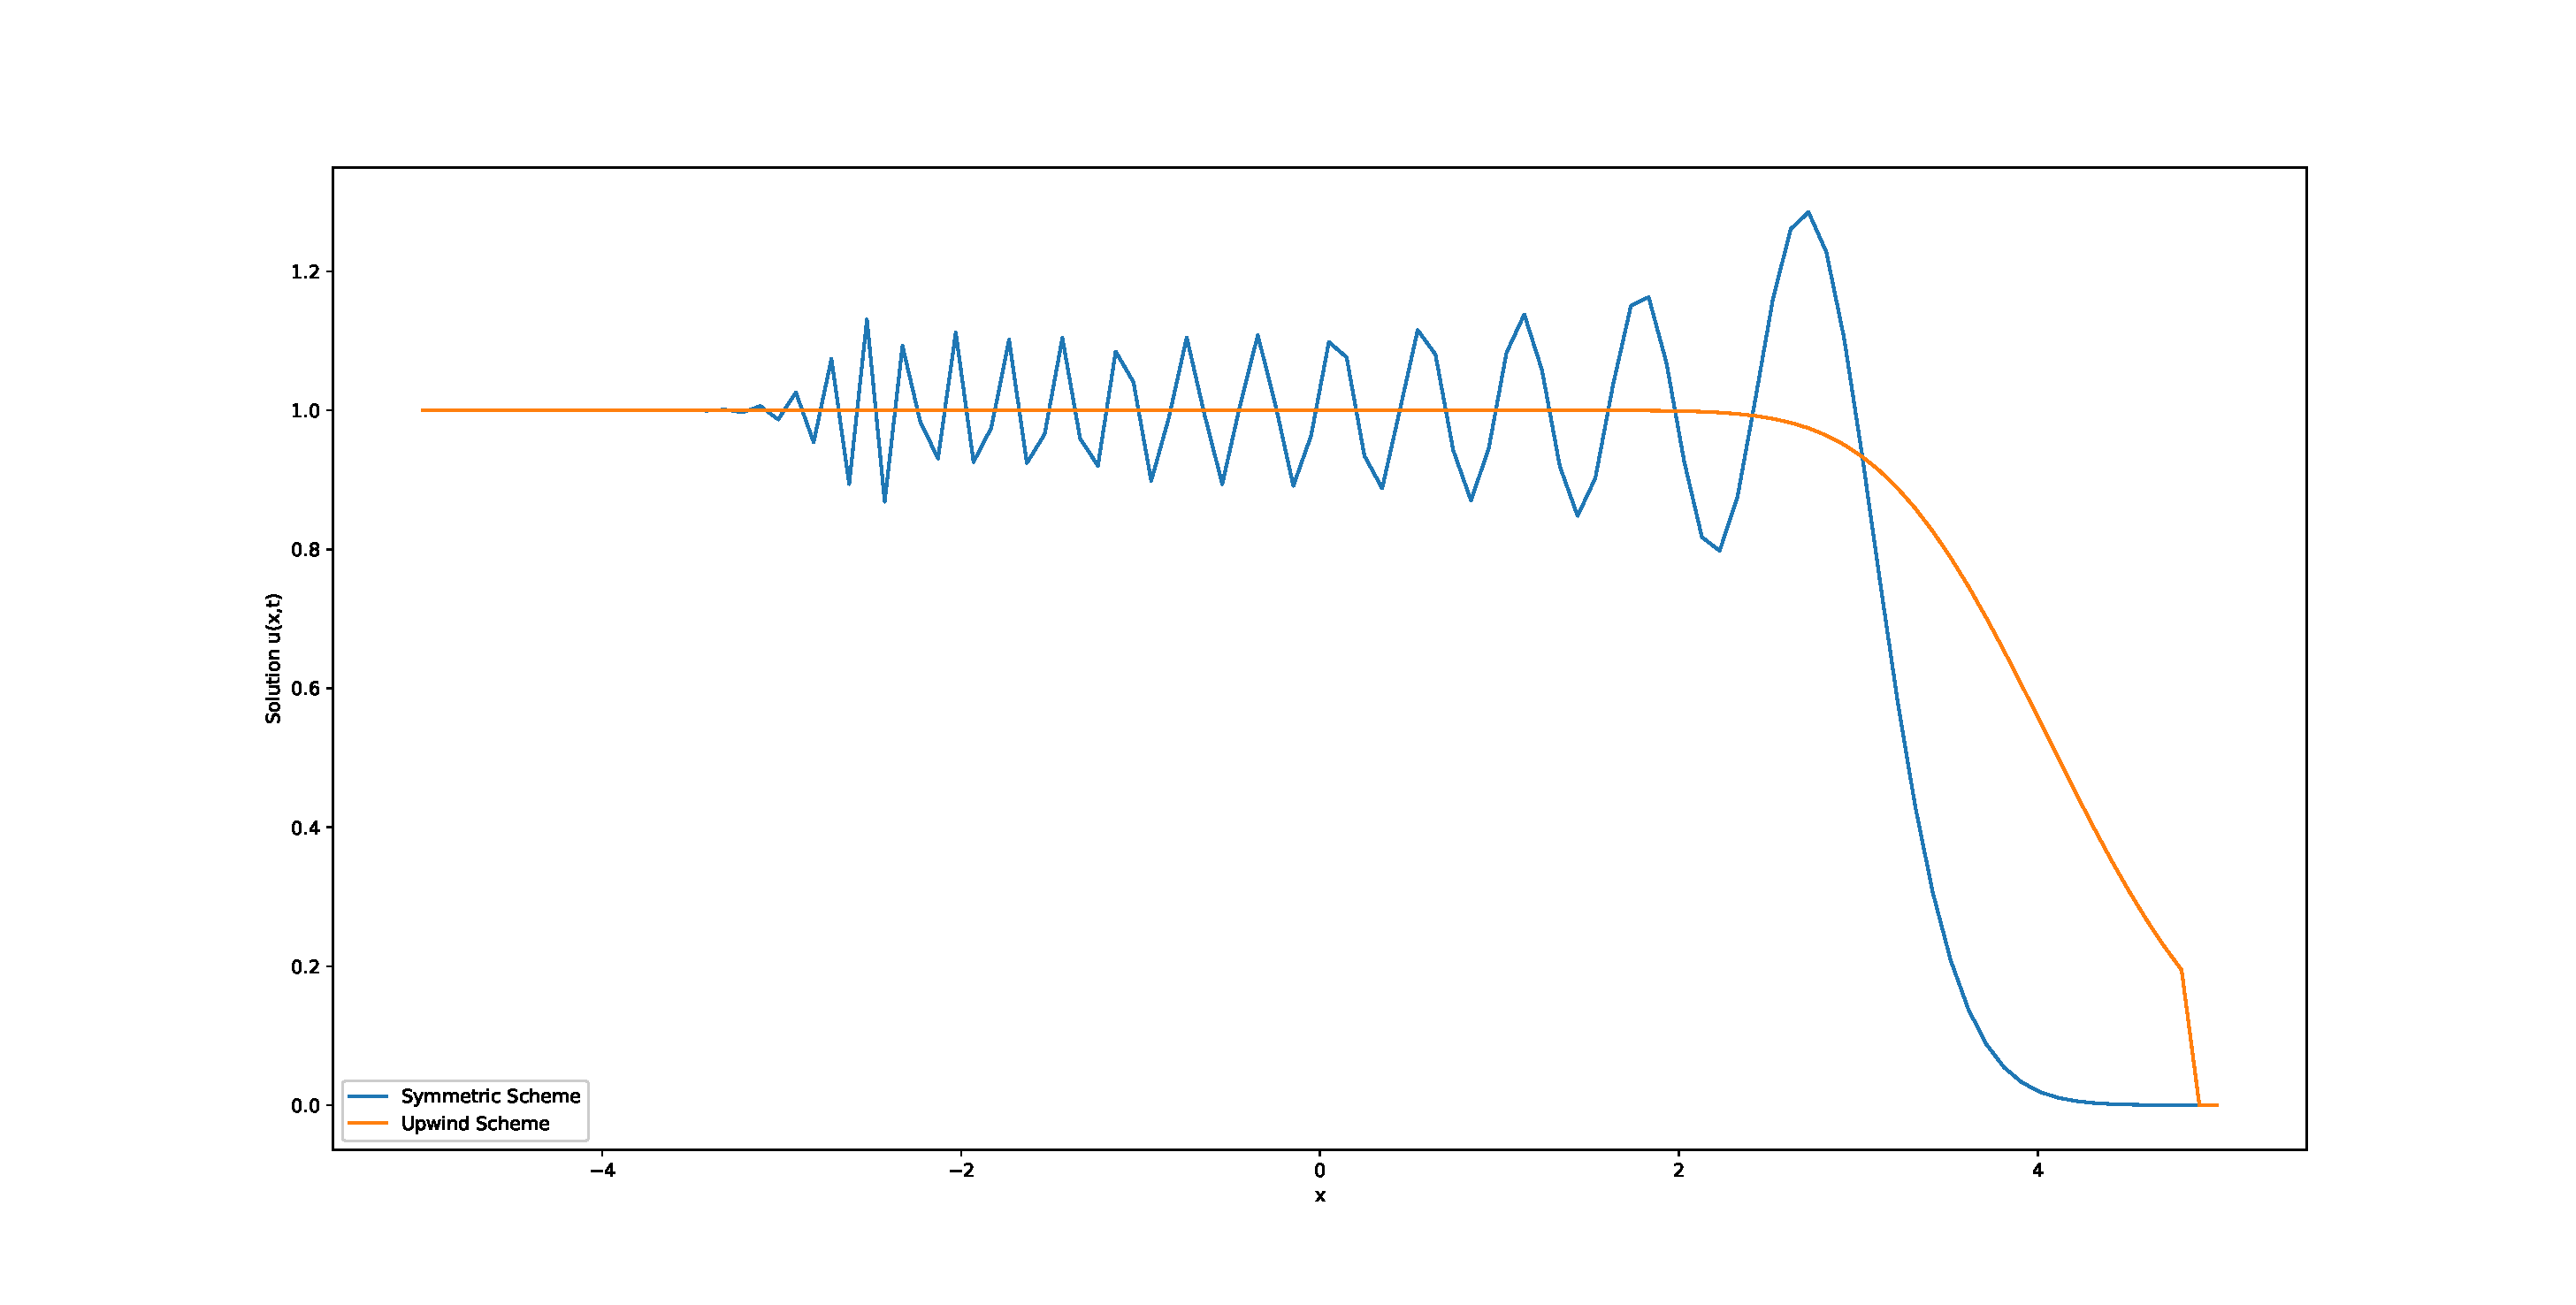
\includegraphics[width=1.0\linewidth]{Plots/symmetric_and_upwind}
	\caption{Plot of the behavior of the symmetric and upwind algorithm for 100 timesteps, right boundary = 1 and left boundary = 0.}
	\label{fig:symmetricandupwind}
\end{figure}

\begin{figure}[H]
	\centering
	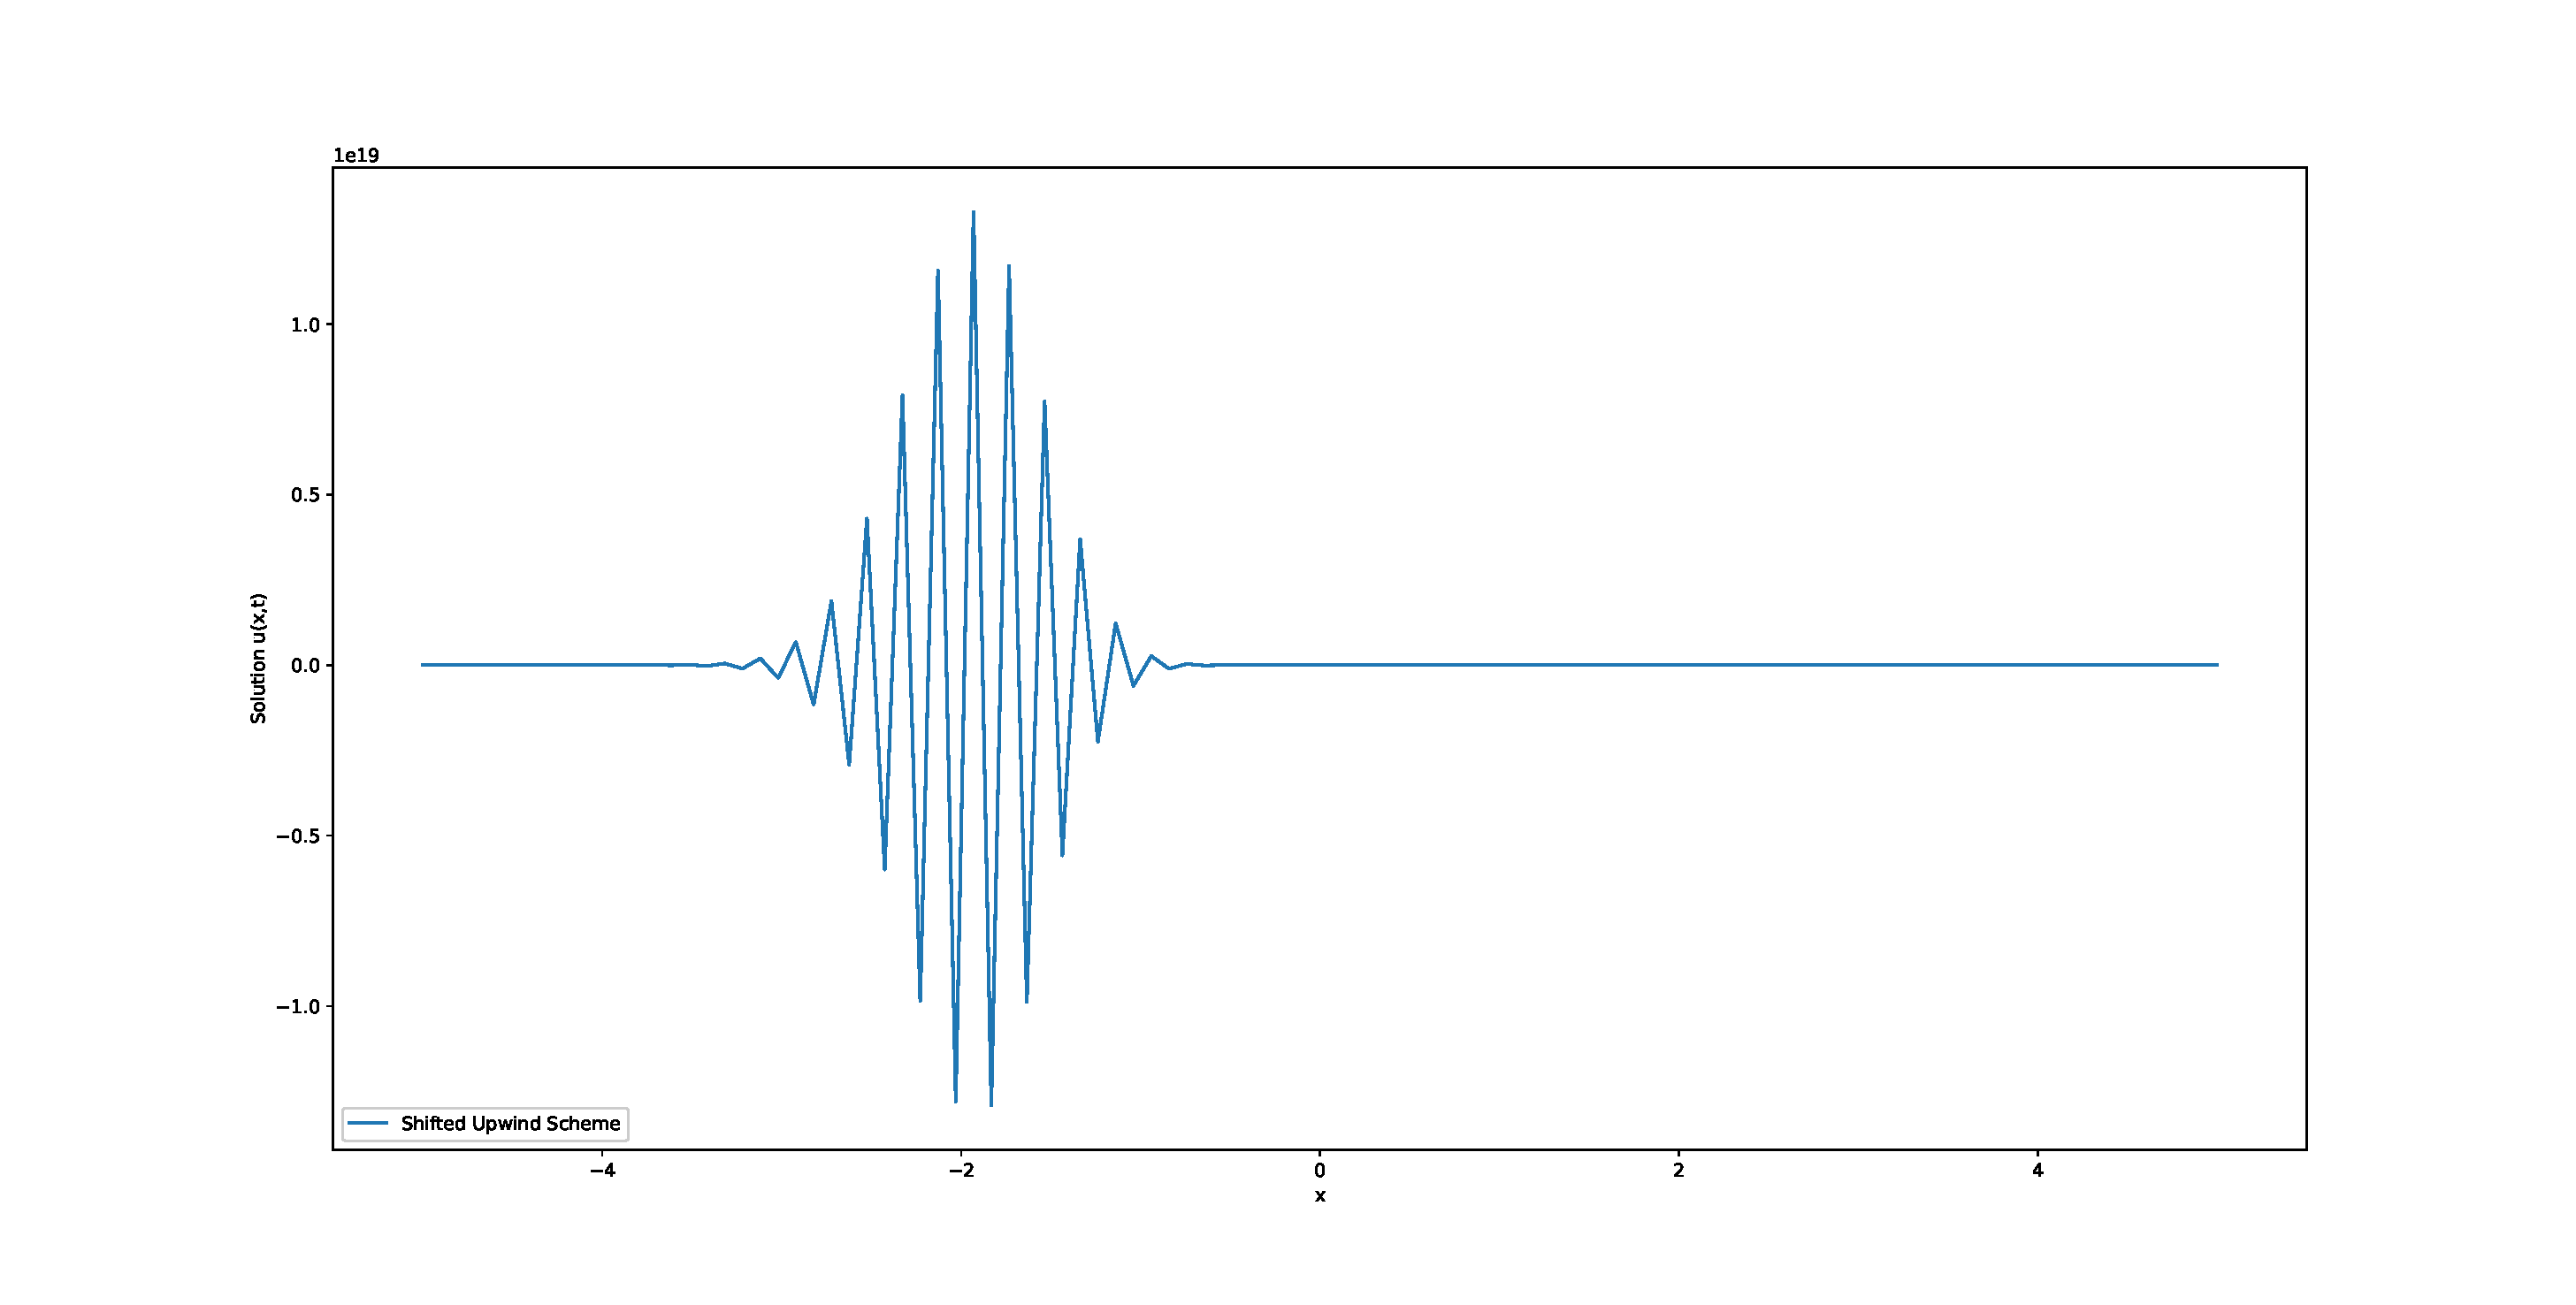
\includegraphics[width=0.8\linewidth]{Plots/upwind_unstable}
	\caption{Plot of the unstable upwind algorithm. One can again immediately see the oscillatory pattern with very large amplitudes compared to the initial condition.}
	\label{fig:upwindunstable}
\end{figure}

Now, we do some further analysis with the stable upwind function. We begin with setting the left boundary condition to \( u/(-L/2, t) = 0.5 \). After that, we do the same for with the right boundary set to \(0.5\). The result is shown in \ref{fig:upwindbounds}. \\
When the left boundary is modified, we see a constant piece at 0.5 followed by a smooth increase to the value 1 and a final decrease to the value 0. The first constant piece at 0.5 is due to the left boundary, because the boundary condition is propagated to the right. We can explain the increase to 1 by the initial condition and its propagation through time. The dip in the end arises from the fact that the initial condition and the information have not been propagated far enough. \\
In a similar manner, we can explain the constant piece at 1 for the modified right boundary. The peak in the end is due to the boundary condition. The constant piece is again due to the propagation of the initial condition and the boundary condition.
\begin{figure}[H]
	\centering
	\includegraphics[width=0.9\linewidth]{Plots/upwind_bounds}
	\caption{Plot of the stable upwind algorithm with different boundary conditions.}
	\label{fig:upwindbounds}
\end{figure}
We can analyze both of these boundary cases for different time step amounts. The results are shown below. Figure \ref{fig:upwindt1000} shows the evolution for 3 seconds sliced into 1000 time steps. We immediately see, that the information was propagated the same distance, which makes sense because the same amount of time has passed, but the result is much smoother, especially in the domain around \( t = 3 \).
\begin{figure}[H]
	\centering
	\includegraphics[width=0.9\linewidth]{Plots/upwind_t1000}
	\caption{Plot of the stable upwind algorithm with 1000 time steps.}
	\label{fig:upwindt1000}
\end{figure}
When we begin to decrease the step amount to 10 steps, we find an entirely different behavior, which is displayed for both boundary conditions in figures \ref{fig:upwindblowupleft} and \ref{fig:upwindblowupright}.
In the domain around \( t = 3\), we get and exponential increase(decrease) for the solution. \\It is blowing up.
The reason for this is that the \textit{Courant-Friedrichs-Levy} criterion is no longer satisfied, because we have \( h = \frac{L}{N} \), where \( N = 100 \) is the cell size and \( L = 10 \) is the length of the system. Then we see that with \( v = 1 \), the CFL-limit is given as \( \Delta t \ll \frac{h}{v} = \frac{1}{10}\), while the systems time step size equals \( \frac{3}{10} \).


\begin{figure}[H]
	\centering
	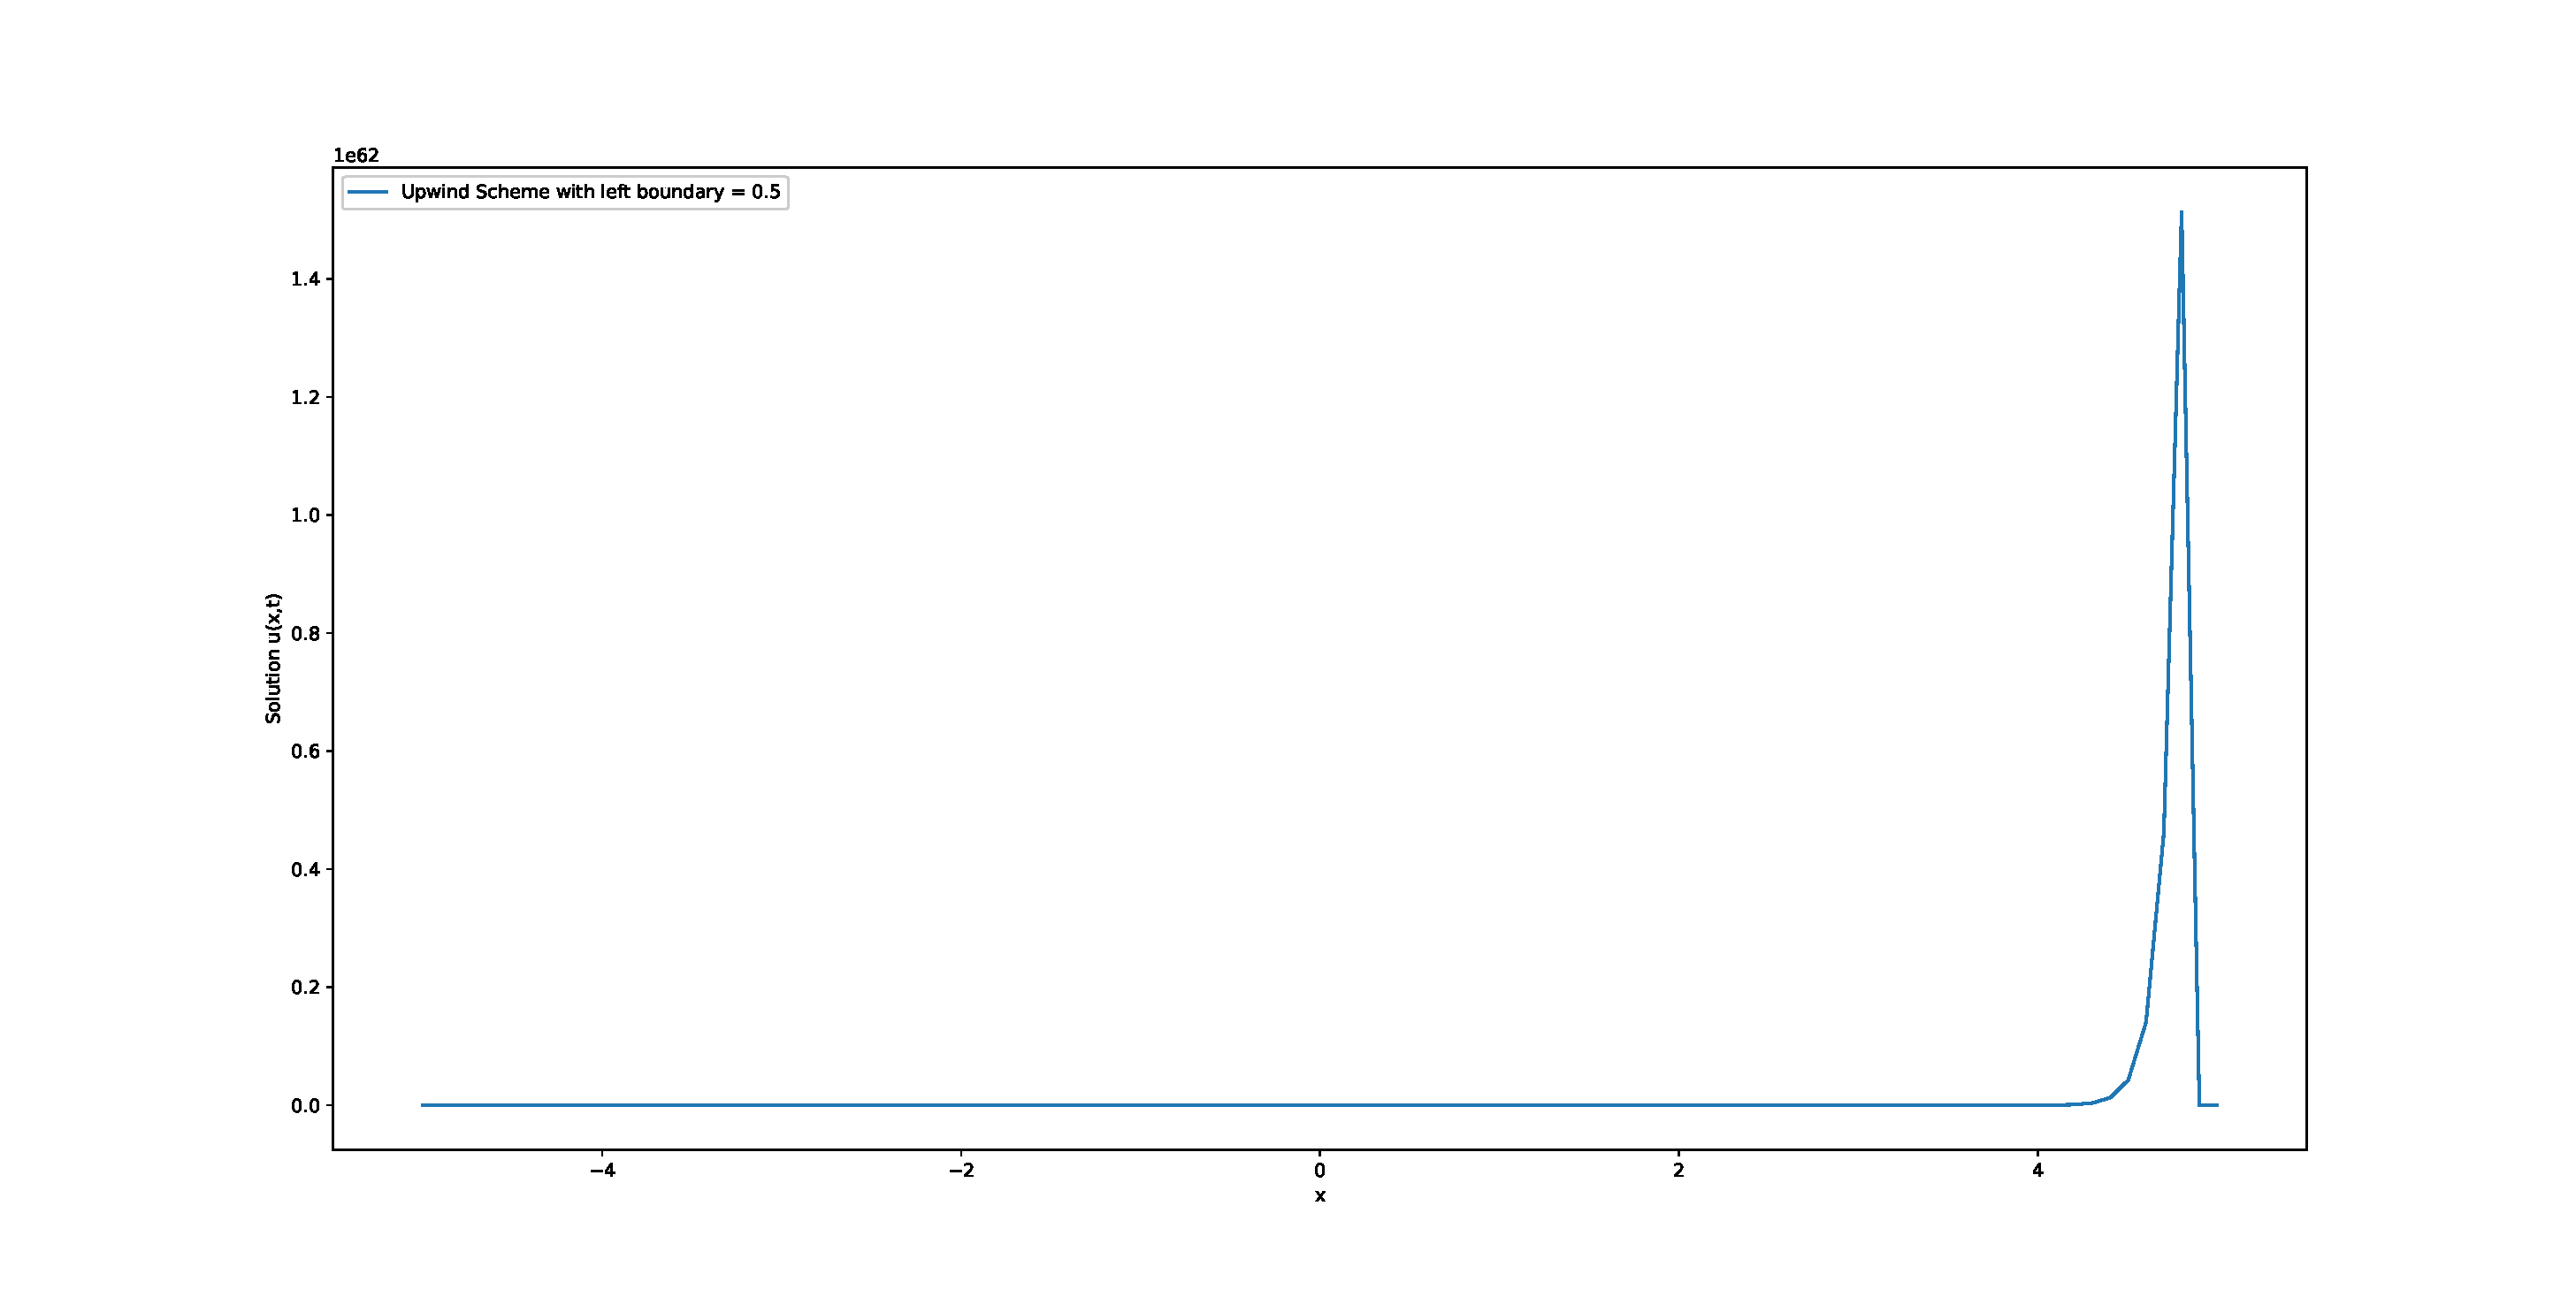
\includegraphics[width=1\linewidth]{Plots/upwind_blowup_left}
	\caption{}
	\label{fig:upwindblowupleft}
\end{figure}

\begin{figure}[H]
	\centering
	\includegraphics[width=1\linewidth]{Plots/upwind_blowup_right}
	\caption{}
	\label{fig:upwindblowupright}
\end{figure}

\newpage

\section*{Exercise 1.2}

The following scheme was used to allow for velocity fields with spatial dependence:
\begin{lstlisting}[title=Function that returns the velocity fields for the different cases.,  language=Python, frame=single]
# Function to create the velocity field for Ex 1.2 with given initial conditions
def velocity(shape, dimension):
	v = np.zeros((dimension + 1, 1))
	if shape == 'constant':
		v = np.ones((dimension + 1, 1))
	if shape == 'linear_convergence':
		for i in range(0, dimension + 1):
	v[i] = -2*(i*dx - L/2) / L
	return v
\end{lstlisting}
\begin{lstlisting}[title=Implementation of a single advection step.,  language=Python, frame=single]
# Function to perform an advection step in Ex1.2
def advect(u, dim, shape):
	v = velocity(shape='constant', dimension=dim)
	for j in range(1, dim):
		u[j] = u[j] - v[j] * (u[j] - u[j - 1]) / dx * dt
	return u
\end{lstlisting}
\begin{lstlisting}[title=Function to perform the advection steps.,  language=Python, frame=single]
# Function to run the advection subroutine
def run_advection(shape, initial_condition=None):
	u, dim = create_field(100, 1, 0, L)
	if initial_condition == 'top_hat':
		u, dim = create_top_hat_field(100, L)
	for i in range(0, timesteps):
		u = advect(u, dim, shape)
	return u
\end{lstlisting}
If we use the initial and boundary conditions given in exercise 1.1, we arrive at the same output as can be seen in figure \ref{fig:upwindnew}.

\begin{figure}[H]
	\centering
	\includegraphics[width=1\linewidth]{Plots/upwind_new}
	\caption{Ouput of the new general-purpose advection function for boundary conditions from exercise 1.1. It is the same as in figure \ref{fig:symmetricandupwind}.}
	\label{fig:upwindnew}
\end{figure}

Using the initial and boundary conditions given in exercise 1.2, we arrive at the time-evolution that is displayed in figures \ref{fig:upwindnewt1000}, \ref{fig:upwindnewt100} and \ref{fig:upwindnewt10}. It shows that the top-hat function is evolved to the right in time. This is not a perfect fit though as the edges of the function are smoothed out. This smoothing-out effect comes from the leftmost and rightmost part of the initial condition, where the function is zero in the beginning. This information is also propagated upstream and causes the smoothing.

\begin{figure}[H]
	\centering
	\includegraphics[width=1\linewidth]{Plots/upwind_new_t1000}
	\caption{Plot of  the general purpose advection subroutine shortly after the beginning.}
	\label{fig:upwindnewt1000}
\end{figure}

\begin{figure}[H]
	\centering
	\includegraphics[width=1\linewidth]{Plots/upwind_new_t100}
	\caption{Plot of  the general purpose advection subroutine after some time has passed.}
	\label{fig:upwindnewt100}
\end{figure}

\begin{figure}[H]
	\centering
	\includegraphics[width=1\linewidth]{Plots/upwind_new_t10}
	\caption{Plot of  the general purpose advection subroutine shortly before it vanishes.}
	\label{fig:upwindnewt10}
\end{figure}



\end{document}
